Recall that polynomial regression learns a function $h_{\bm{\theta}}(x) = \theta_0 + \theta_1 x + \theta_2 x^2 + \ldots + \theta_d x^d$.  In this case, $d$ represents the polynomial's degree.  We can equivalently write this in the form of a  linear model
\begin{equation}
h_{\bm{\theta}}(x) = \theta_0 \phi_0(x) + \theta_1 \phi_1(x)  + \theta_2 \phi_2(x)  + \ldots + \theta_d \phi_d(x)  \enspace ,
\end{equation}
using the basis expansion that $\phi_j(x) = x^j$.  Notice that, with this basis expansion, we obtain a linear model where the features are various powers of the single univariate $x$.  We're still solving a linear regression problem, but are fitting a polynomial function of the input.\\

 Implement regularized polynomial regression in \texttt{polyreg.py}.  You may implement it however you like, using gradient descent or a closed-form solution.  However, I would recommend the closed-form solution since the data sets are small; for this reason, we've included an example closed-form implementation of linear regression in \texttt{linreg\_closedform.py} (you are welcome to build upon this implementation, but make CERTAIN you understand it, since you'll need to change several lines of it).  You are also welcome to build upon your implementation from the previous assignment, but you must follow the API below.  Note that all matrices are actually 2D numpy arrays in the implementation.\\

\begin{itemize}[noitemsep, nolistsep]
    \item \texttt{\_\_init\_\_(degree=1, regLambda=1E-8)} : constructor with arguments of $d$ and $\lambda$
    \item \texttt{fit(X,Y)}: method to train the polynomial regression model
    \item \texttt{predict(X)}: method to use the trained polynomial regression model for prediction
    \item \texttt{polyfeatures(X, degree)}: expands the given $n \times 1$ matrix $X$ into an $n \times d$ matrix of polynomial features of degree $d$.  Note that the returned matrix will not include the zero-th power.
\end{itemize}

Note that the \texttt{polyfeatures(X, degree)} function maps the original univariate data into its higher order powers.  Specifically, $X$ will be an $n \times 1$ matrix $(X \in \mathbb{R}^{n \times 1})$ and this function will return the polynomial expansion of this data, a $n \times d$ matrix.  Note that this function will {\bf not} add in the zero-th order feature (i.e., $x_0 = 1$).  You should add the $x_0$ feature separately, outside of this function, before training the model.
\begin{wrapfigure}{r}{0.42\textwidth}
  \centering
  \vspace{-1em}
  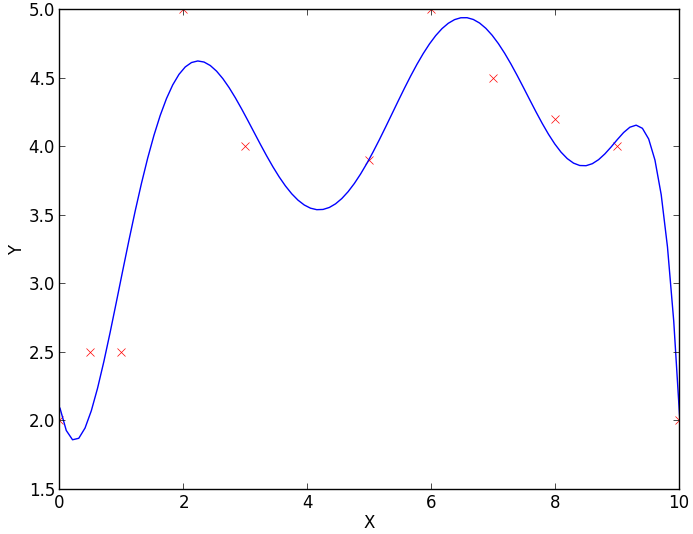
\includegraphics[width=0.4\textwidth]{images/polyregDegree8.png}
    \vspace{-1em}
  \caption{Fit of polynomial regression with $\lambda = 0$ and $d = 8$}\label{fig:polyregUnivariate}
  \vspace{-2em}
\end{wrapfigure}
By not including the $x_0$ column in the matrix \texttt{polyfeatures()}, this allows the \texttt{polyfeatures} function to be more general, so it could be applied to multi-variate data as well. (If it did add the $x_0$ feature, we'd end up with multiple columns of 1's for multivariate data.)\\

Also, notice that the resulting features will be badly scaled if we use them in raw form.  For example, with a polynomial of degree $d = 8$ and $x = 20$, the basis expansion yields $x^1 = 20$ while $x^8 = 2.56 \times 10^{10}$ -- an
absolutely huge difference in range.  Consequently, we will need to standardize the data before solving linear regression.  Standardize the data in \texttt{fit()} after you perform the polynomial feature expansion.  You'll need to apply the same standardization transformation in \texttt{predict()} before you apply it to new data.\\

 Run \texttt{test\_polyreg\_univariate.py} to test your implementation, which will plot the learned function.  In this case, the script fits a polynomial of degree $d=8$ with no regularization $\lambda = 0$.  From the plot, we see that the function fits the data well, but will not generalize well to new data points.  Try increasing the amount of regularization, and examine the resulting effect on the function.\\

\begin{quote}
    \FloatBarrier
    \begin{figure}
	\captionsetup{labelformat=empty}
	\caption{Results of training Polynomial Regression model of degree d = 8.}
   	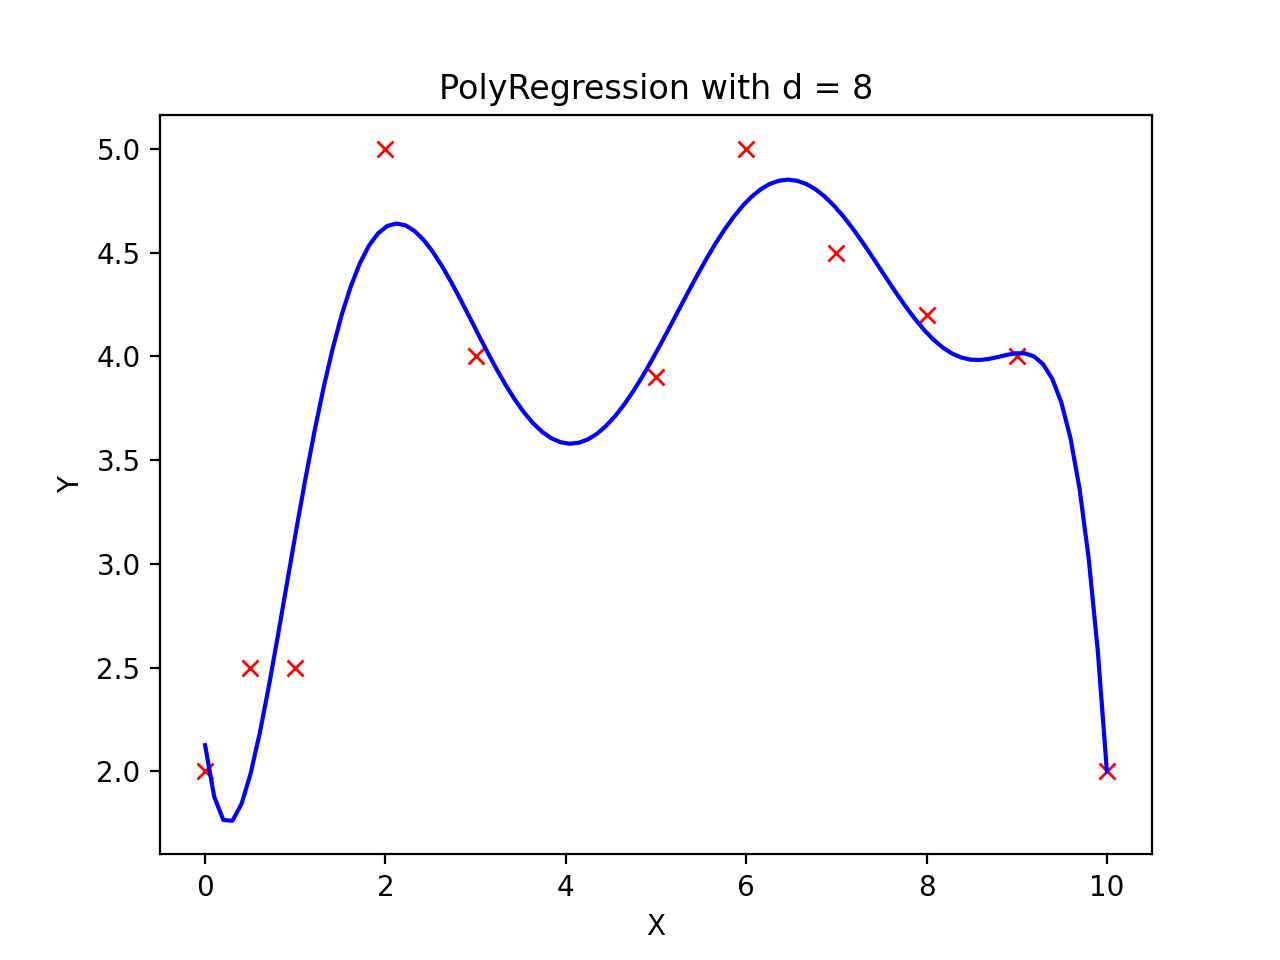
\includegraphics[scale=0.5]{./images/fig1.png} 
	\centering
    \end{figure}
    \FloatBarrier
\end{quote}

